\documentclass{standalone}
\usepackage{tikz}
\usetikzlibrary{patterns, positioning}


\begin{document}
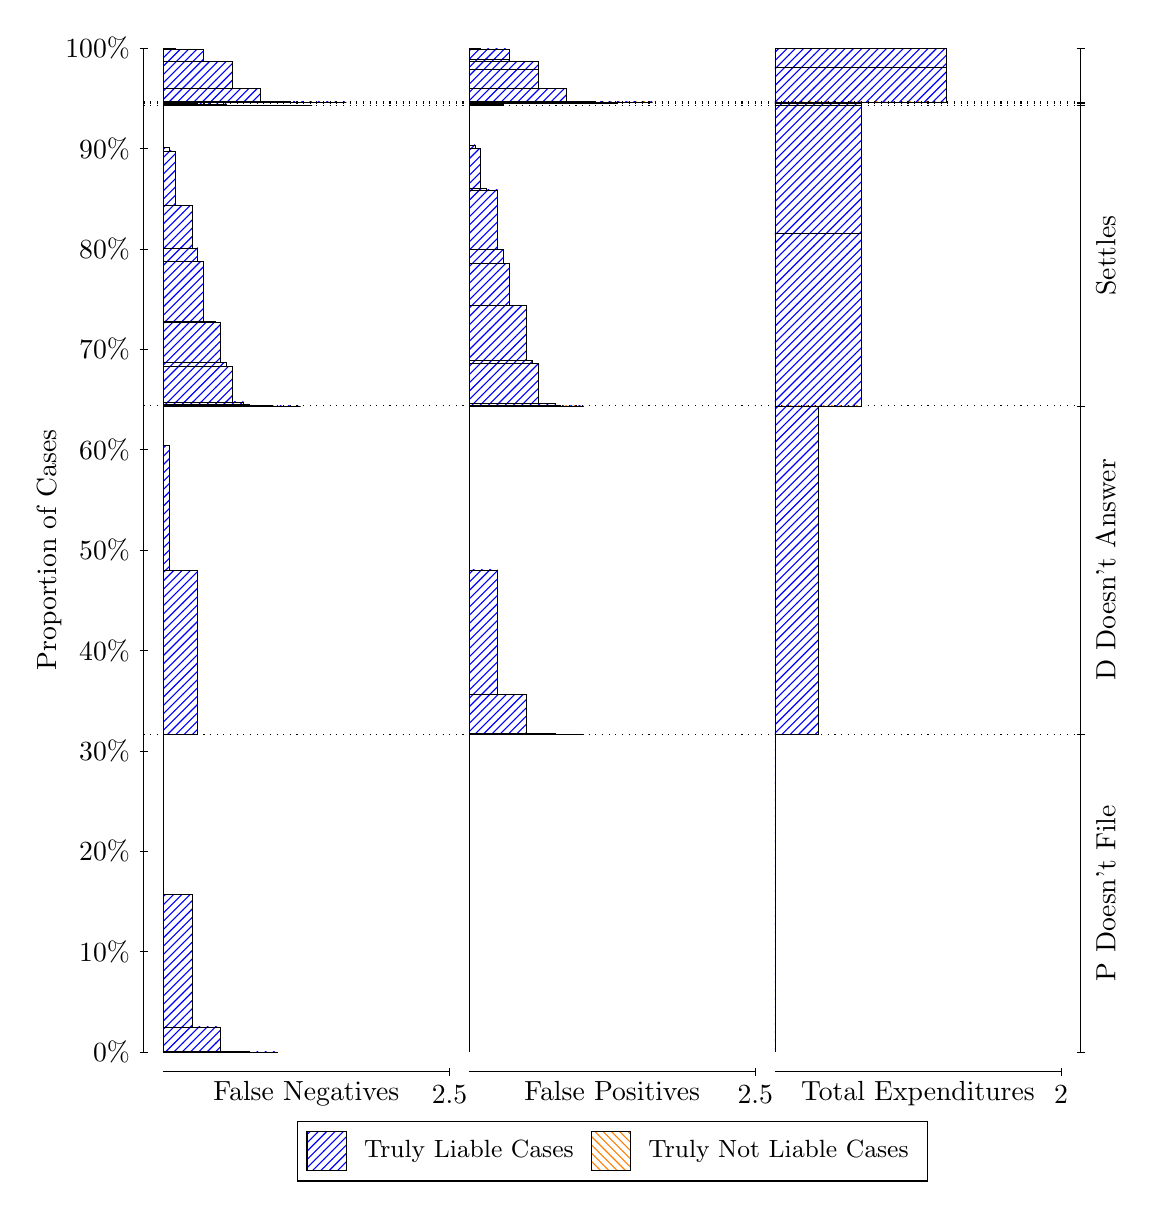
\begin{tikzpicture}
\draw[black, very thin] (1.5,1.75) -- (1.5,14.5);
\node[rotate=90, text=black, anchor=center] at (0.3, 8.125) {Proportion of Cases};
\draw[black, very thin] (1.45,1.75) -- (1.55,1.75);
\node[text=black, anchor=east] at (1.45, 1.75) {0\%};
\draw[black, very thin] (1.45,3.025) -- (1.55,3.025);
\node[text=black, anchor=east] at (1.45, 3.025) {10\%};
\draw[black, very thin] (1.45,4.3) -- (1.55,4.3);
\node[text=black, anchor=east] at (1.45, 4.3) {20\%};
\draw[black, very thin] (1.45,5.575) -- (1.55,5.575);
\node[text=black, anchor=east] at (1.45, 5.575) {30\%};
\draw[black, very thin] (1.45,6.85) -- (1.55,6.85);
\node[text=black, anchor=east] at (1.45, 6.85) {40\%};
\draw[black, very thin] (1.45,8.125) -- (1.55,8.125);
\node[text=black, anchor=east] at (1.45, 8.125) {50\%};
\draw[black, very thin] (1.45,9.4) -- (1.55,9.4);
\node[text=black, anchor=east] at (1.45, 9.4) {60\%};
\draw[black, very thin] (1.45,10.675) -- (1.55,10.675);
\node[text=black, anchor=east] at (1.45, 10.675) {70\%};
\draw[black, very thin] (1.45,11.95) -- (1.55,11.95);
\node[text=black, anchor=east] at (1.45, 11.95) {80\%};
\draw[black, very thin] (1.45,13.225) -- (1.55,13.225);
\node[text=black, anchor=east] at (1.45, 13.225) {90\%};
\draw[black, very thin] (1.45,14.5) -- (1.55,14.5);
\node[text=black, anchor=east] at (1.45, 14.5) {100\%};

\draw[black, very thin] (13.4,1.75) -- (13.4,14.5);
\draw[black, very thin] (13.35,1.75) -- (13.45,1.75);
\node[anchor=west] at (13.35, 1.75) {};
\draw[black, very thin] (13.35,5.7845) -- (13.45,5.7845);
\node[anchor=west] at (13.35, 5.7845) {};
\draw[black, very thin] (13.35,9.9564) -- (13.45,9.9564);
\node[anchor=west] at (13.35, 9.9564) {};
\draw[black, very thin] (13.35,13.773) -- (13.45,13.773);
\node[anchor=west] at (13.35, 13.773) {};
\draw[black, very thin] (13.35,13.798) -- (13.45,13.798);
\node[anchor=west] at (13.35, 13.798) {};
\draw[black, very thin] (13.35,13.815) -- (13.45,13.815);
\node[anchor=west] at (13.35, 13.815) {};
\draw[black, very thin] (13.35,14.5) -- (13.45,14.5);
\node[anchor=west] at (13.35, 14.5) {};

\draw[black, very thin, pattern color=blue, pattern=north east lines] (1.75,1.75) rectangle (3.2033,1.75);
\draw[black, very thin, pattern color=blue, pattern=north east lines] (1.75,1.75) rectangle (2.84,1.7527);
\draw[black, very thin, pattern color=blue, pattern=north east lines] (1.75,1.7527) rectangle (2.4767,2.0696);
\draw[black, very thin, pattern color=blue, pattern=north east lines] (1.75,2.0696) rectangle (2.1133,3.7559);
\draw[black, very thin, pattern color=orange, pattern=north west lines] (1.75,3.7559) rectangle (1.75,3.7559);
\draw[black, very thin, pattern color=blue, pattern=north east lines] (1.75,3.7559) rectangle (1.75,5.7845);
\draw[black, very thin, pattern color=blue, pattern=north east lines] (1.75,5.7845) rectangle (2.186,7.8691);
\draw[black, very thin, pattern color=blue, pattern=north east lines] (1.75,7.8691) rectangle (1.8227,9.4529);
\draw[black, very thin, pattern color=orange, pattern=north west lines] (1.75,9.4529) rectangle (1.75,9.4529);
\draw[black, very thin, pattern color=blue, pattern=north east lines] (1.75,9.4529) rectangle (1.75,9.9564);
\draw[black, very thin, pattern color=blue, pattern=north east lines] (1.75,9.9564) rectangle (3.494,9.9564);
\draw[black, very thin, pattern color=blue, pattern=north east lines] (1.75,9.9564) rectangle (3.2033,9.9564);
\draw[black, very thin, pattern color=blue, pattern=north east lines] (1.75,9.9564) rectangle (3.1307,9.9571);
\draw[black, very thin, pattern color=blue, pattern=north east lines] (1.75,9.9571) rectangle (2.9127,9.9582);
\draw[black, very thin, pattern color=blue, pattern=north east lines] (1.75,9.9582) rectangle (2.84,9.9775);
\draw[black, very thin, pattern color=blue, pattern=north east lines] (1.75,9.9775) rectangle (2.7673,10.005);
\draw[black, very thin, pattern color=blue, pattern=north east lines] (1.75,10.005) rectangle (2.622,10.46);
\draw[black, very thin, pattern color=blue, pattern=north east lines] (1.75,10.46) rectangle (2.5493,10.506);
\draw[black, very thin, pattern color=blue, pattern=north east lines] (1.75,10.506) rectangle (2.4767,11.012);
\draw[black, very thin, pattern color=blue, pattern=north east lines] (1.75,11.012) rectangle (2.404,11.033);
\draw[black, very thin, pattern color=blue, pattern=north east lines] (1.75,11.033) rectangle (2.2587,11.79);
\draw[black, very thin, pattern color=blue, pattern=north east lines] (1.75,11.79) rectangle (2.186,11.962);
\draw[black, very thin, pattern color=blue, pattern=north east lines] (1.75,11.962) rectangle (2.1133,12.502);
\draw[black, very thin, pattern color=blue, pattern=north east lines] (1.75,12.502) rectangle (2.0407,12.503);
\draw[black, very thin, pattern color=blue, pattern=north east lines] (1.75,12.503) rectangle (1.8953,13.193);
\draw[black, very thin, pattern color=blue, pattern=north east lines] (1.75,13.193) rectangle (1.8227,13.236);
\draw[black, very thin, pattern color=orange, pattern=north west lines] (1.75,13.236) rectangle (1.75,13.236);
\draw[black, very thin, pattern color=blue, pattern=north east lines] (1.75,13.236) rectangle (1.75,13.773);
\draw[black, very thin, pattern color=blue, pattern=north east lines] (1.75,13.773) rectangle (3.6393,13.773);
\draw[black, very thin, pattern color=blue, pattern=north east lines] (1.75,13.773) rectangle (3.276,13.773);
\draw[black, very thin, pattern color=blue, pattern=north east lines] (1.75,13.773) rectangle (2.9127,13.775);
\draw[black, very thin, pattern color=blue, pattern=north east lines] (1.75,13.775) rectangle (2.5493,13.79);
\draw[black, very thin, pattern color=blue, pattern=north east lines] (1.75,13.79) rectangle (2.186,13.798);
\draw[black, very thin, pattern color=orange, pattern=north west lines] (1.75,13.798) rectangle (1.75,13.798);
\draw[black, very thin, pattern color=blue, pattern=north east lines] (1.75,13.798) rectangle (2.186,13.805);
\draw[black, very thin, pattern color=blue, pattern=north east lines] (1.75,13.805) rectangle (1.8227,13.815);
\draw[black, very thin, pattern color=orange, pattern=north west lines] (1.75,13.815) rectangle (1.75,13.815);
\draw[black, very thin, pattern color=blue, pattern=north east lines] (1.75,13.815) rectangle (1.75,13.815);
\draw[black, very thin, pattern color=blue, pattern=north east lines] (1.75,13.815) rectangle (4.0753,13.815);
\draw[black, very thin, pattern color=blue, pattern=north east lines] (1.75,13.815) rectangle (3.712,13.815);
\draw[black, very thin, pattern color=blue, pattern=north east lines] (1.75,13.815) rectangle (3.3487,13.826);
\draw[black, very thin, pattern color=blue, pattern=north east lines] (1.75,13.826) rectangle (2.9853,13.984);
\draw[black, very thin, pattern color=blue, pattern=north east lines] (1.75,13.984) rectangle (2.622,14.328);
\draw[black, very thin, pattern color=blue, pattern=north east lines] (1.75,14.328) rectangle (2.2587,14.487);
\draw[black, very thin, pattern color=blue, pattern=north east lines] (1.75,14.487) rectangle (1.8953,14.5);
\draw[black, very thin, pattern color=orange, pattern=north west lines] (1.75,14.5) rectangle (1.75,14.5);
\draw[black, very thin, pattern color=blue, pattern=north east lines] (1.75,14.5) rectangle (1.75,14.5);
\draw[black, very thin, pattern color=orange, pattern=north west lines] (5.6333,1.75) rectangle (5.6333,1.75);
\draw[black, very thin, pattern color=blue, pattern=north east lines] (5.6333,1.75) rectangle (5.6333,5.7845);
\draw[black, very thin, pattern color=orange, pattern=north west lines] (5.6333,5.7845) rectangle (7.0867,5.7845);
\draw[black, very thin, pattern color=blue, pattern=north east lines] (5.6333,5.7845) rectangle (7.0867,5.7845);
\draw[black, very thin, pattern color=blue, pattern=north east lines] (5.6333,5.7845) rectangle (6.7233,5.7963);
\draw[black, very thin, pattern color=blue, pattern=north east lines] (5.6333,5.7963) rectangle (6.36,6.288);
\draw[black, very thin, pattern color=blue, pattern=north east lines] (5.6333,6.288) rectangle (5.9967,7.8718);
\draw[black, very thin, pattern color=blue, pattern=north east lines] (5.6333,7.8718) rectangle (5.6333,9.9564);
\draw[black, very thin, pattern color=orange, pattern=north west lines] (5.6333,9.9564) rectangle (7.0867,9.9564);
\draw[black, very thin, pattern color=blue, pattern=north east lines] (5.6333,9.9564) rectangle (7.0867,9.9564);
\draw[black, very thin, pattern color=orange, pattern=north west lines] (5.6333,9.9564) rectangle (6.796,9.9564);
\draw[black, very thin, pattern color=blue, pattern=north east lines] (5.6333,9.9564) rectangle (6.796,9.9575);
\draw[black, very thin, pattern color=blue, pattern=north east lines] (5.6333,9.9575) rectangle (6.7233,9.9832);
\draw[black, very thin, pattern color=orange, pattern=north west lines] (5.6333,9.9832) rectangle (6.5053,9.9832);
\draw[black, very thin, pattern color=blue, pattern=north east lines] (5.6333,9.9832) rectangle (6.5053,10.493);
\draw[black, very thin, pattern color=blue, pattern=north east lines] (5.6333,10.493) rectangle (6.4327,10.536);
\draw[black, very thin, pattern color=blue, pattern=north east lines] (5.6333,10.536) rectangle (6.36,11.227);
\draw[black, very thin, pattern color=orange, pattern=north west lines] (5.6333,11.227) rectangle (6.2147,11.227);
\draw[black, very thin, pattern color=blue, pattern=north east lines] (5.6333,11.227) rectangle (6.2147,11.227);
\draw[black, very thin, pattern color=blue, pattern=north east lines] (5.6333,11.227) rectangle (6.142,11.768);
\draw[black, very thin, pattern color=blue, pattern=north east lines] (5.6333,11.768) rectangle (6.0693,11.939);
\draw[black, very thin, pattern color=blue, pattern=north east lines] (5.6333,11.939) rectangle (5.9967,12.697);
\draw[black, very thin, pattern color=blue, pattern=north east lines] (5.6333,12.697) rectangle (5.8513,12.718);
\draw[black, very thin, pattern color=blue, pattern=north east lines] (5.6333,12.718) rectangle (5.7787,13.223);
\draw[black, very thin, pattern color=blue, pattern=north east lines] (5.6333,13.223) rectangle (5.706,13.269);
\draw[black, very thin, pattern color=blue, pattern=north east lines] (5.6333,13.269) rectangle (5.6333,13.773);
\draw[black, very thin, pattern color=orange, pattern=north west lines] (5.6333,13.773) rectangle (6.0693,13.773);
\draw[black, very thin, pattern color=blue, pattern=north east lines] (5.6333,13.773) rectangle (6.0693,13.78);
\draw[black, very thin, pattern color=blue, pattern=north east lines] (5.6333,13.78) rectangle (5.706,13.796);
\draw[black, very thin, pattern color=blue, pattern=north east lines] (5.6333,13.796) rectangle (5.6333,13.798);
\draw[black, very thin, pattern color=orange, pattern=north west lines] (5.6333,13.798) rectangle (7.5227,13.798);
\draw[black, very thin, pattern color=blue, pattern=north east lines] (5.6333,13.798) rectangle (7.5227,13.798);
\draw[black, very thin, pattern color=blue, pattern=north east lines] (5.6333,13.798) rectangle (7.1593,13.798);
\draw[black, very thin, pattern color=blue, pattern=north east lines] (5.6333,13.798) rectangle (6.796,13.798);
\draw[black, very thin, pattern color=blue, pattern=north east lines] (5.6333,13.798) rectangle (6.4327,13.808);
\draw[black, very thin, pattern color=blue, pattern=north east lines] (5.6333,13.808) rectangle (6.0693,13.815);
\draw[black, very thin, pattern color=orange, pattern=north west lines] (5.6333,13.815) rectangle (7.9587,13.815);
\draw[black, very thin, pattern color=blue, pattern=north east lines] (5.6333,13.815) rectangle (7.9587,13.815);
\draw[black, very thin, pattern color=orange, pattern=north west lines] (5.6333,13.815) rectangle (7.5953,13.815);
\draw[black, very thin, pattern color=blue, pattern=north east lines] (5.6333,13.815) rectangle (7.5953,13.815);
\draw[black, very thin, pattern color=orange, pattern=north west lines] (5.6333,13.815) rectangle (7.232,13.815);
\draw[black, very thin, pattern color=blue, pattern=north east lines] (5.6333,13.815) rectangle (7.232,13.827);
\draw[black, very thin, pattern color=blue, pattern=north east lines] (5.6333,13.827) rectangle (6.8687,13.986);
\draw[black, very thin, pattern color=orange, pattern=north west lines] (5.6333,13.986) rectangle (6.8687,13.986);
\draw[black, very thin, pattern color=blue, pattern=north east lines] (5.6333,13.986) rectangle (6.8687,13.987);
\draw[black, very thin, pattern color=blue, pattern=north east lines] (5.6333,13.987) rectangle (6.5053,14.224);
\draw[black, very thin, pattern color=orange, pattern=north west lines] (5.6333,14.224) rectangle (6.5053,14.224);
\draw[black, very thin, pattern color=blue, pattern=north east lines] (5.6333,14.224) rectangle (6.5053,14.33);
\draw[black, very thin, pattern color=blue, pattern=north east lines] (5.6333,14.33) rectangle (6.142,14.362);
\draw[black, very thin, pattern color=blue, pattern=north east lines] (5.6333,14.362) rectangle (6.142,14.489);
\draw[black, very thin, pattern color=blue, pattern=north east lines] (5.6333,14.489) rectangle (5.7787,14.489);
\draw[black, very thin, pattern color=blue, pattern=north east lines] (5.6333,14.489) rectangle (5.7787,14.5);
\draw[black, very thin, pattern color=blue, pattern=north east lines] (5.6333,14.5) rectangle (5.6333,14.5);
\draw[black, very thin, pattern color=orange, pattern=north west lines] (9.5167,1.75) rectangle (9.5167,1.75);
\draw[black, very thin, pattern color=blue, pattern=north east lines] (9.5167,1.75) rectangle (9.5167,5.7845);
\draw[black, very thin, pattern color=orange, pattern=north west lines] (9.5167,5.7845) rectangle (10.062,5.7845);
\draw[black, very thin, pattern color=blue, pattern=north east lines] (9.5167,5.7845) rectangle (10.062,9.9564);
\draw[black, very thin, pattern color=orange, pattern=north west lines] (9.5167,9.9564) rectangle (10.607,9.9564);
\draw[black, very thin, pattern color=blue, pattern=north east lines] (9.5167,9.9564) rectangle (10.607,12.148);
\draw[black, very thin, pattern color=orange, pattern=north west lines] (9.5167,12.148) rectangle (10.607,12.148);
\draw[black, very thin, pattern color=blue, pattern=north east lines] (9.5167,12.148) rectangle (10.607,13.773);
\draw[black, very thin, pattern color=orange, pattern=north west lines] (9.5167,13.773) rectangle (10.607,13.773);
\draw[black, very thin, pattern color=blue, pattern=north east lines] (9.5167,13.773) rectangle (10.607,13.798);
\draw[black, very thin, pattern color=orange, pattern=north west lines] (9.5167,13.798) rectangle (10.607,13.798);
\draw[black, very thin, pattern color=blue, pattern=north east lines] (9.5167,13.798) rectangle (10.607,13.815);
\draw[black, very thin, pattern color=orange, pattern=north west lines] (9.5167,13.815) rectangle (11.697,13.815);
\draw[black, very thin, pattern color=blue, pattern=north east lines] (9.5167,13.815) rectangle (11.697,14.255);
\draw[black, very thin, pattern color=orange, pattern=north west lines] (9.5167,14.255) rectangle (11.697,14.255);
\draw[black, very thin, pattern color=blue, pattern=north east lines] (9.5167,14.255) rectangle (11.697,14.5);
\draw[black, dotted] (1.5,5.7845) -- (13.4,5.7845);
\draw[black, dotted] (1.5,9.9564) -- (13.4,9.9564);
\draw[black, dotted] (1.5,13.773) -- (13.4,13.773);
\draw[black, dotted] (1.5,13.798) -- (13.4,13.798);
\draw[black, dotted] (1.5,13.815) -- (13.4,13.815);
\draw[black, very thin] (1.75,1.5) -- (5.3833,1.5);
\node[text=black, anchor=north] at (3.5667, 1.5) {False Negatives};
\draw[black, very thin] (5.3833,1.45) -- (5.3833,1.55);
\node[text=black, anchor=north] at (5.3833, 1.45) {2.5};

\draw[black, very thin] (5.6333,1.5) -- (9.2667,1.5);
\node[text=black, anchor=north] at (7.45, 1.5) {False Positives};
\draw[black, very thin] (9.2667,1.45) -- (9.2667,1.55);
\node[text=black, anchor=north] at (9.2667, 1.45) {2.5};

\draw[black, very thin] (9.5167,1.5) -- (13.15,1.5);
\node[text=black, anchor=north] at (11.333, 1.5) {Total Expenditures};
\draw[black, very thin] (13.15,1.45) -- (13.15,1.55);
\node[text=black, anchor=north] at (13.15, 1.45) {2};

\node[text=black, centered, rotate=90] at (13.72, 3.7673) {P Doesn't File};
\node[text=black, centered, rotate=90] at (13.72, 7.8705) {D Doesn't Answer};
\node[text=black, centered, rotate=90] at (13.72, 11.865) {Settles};




\draw (7.449999999999999,1.5) node[draw=none] (baseCoordinate) {};
\begin{scope}[align=center]
        \matrix[scale=0.5, draw=black, below=0.5cm of baseCoordinate, nodes={draw}, column sep=0.1cm]{
            \node[rectangle, draw, minimum width=0.5cm, minimum height=0.5cm, pattern color=blue, pattern=north east lines] {}; &
            \node[draw=none, font=\small, text=black] (B) {Truly Liable Cases}; &
            \node[rectangle, draw, minimum width=0.5cm, minimum height=0.5cm, pattern color=orange, pattern=north west lines] {}; &
            \node[draw=none, font=\small, text=black] (B) {Truly Not Liable Cases}; \\
            };
\end{scope}

\end{tikzpicture}
\end{document}